\subsection{Der core-Ordner}
Die Abbildung \ref{fig:core-sturktur} bietet eine Übersicht des \lstinline|core|-Ordnerinhaltes und der inneren Abhängigkeiten.
Dem Anhang ist das Diagram D2\_Core.html beigefügt, welches eine detailliertere Darstellung der Abhängigkeit enthält.
%Die Tabelle \ref{table:coreMap} kategorisiert den Quelltext des Ordners in Bausteine.
\begin{figure}[H]
    \centering
    \caption{Übersicht der Strukturierung des Ordners \lstinline|core|}
    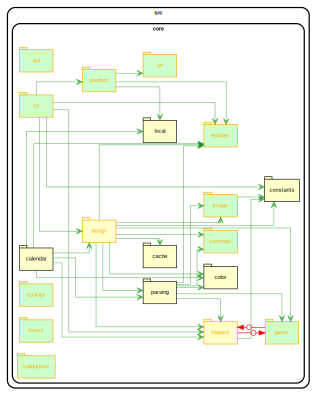
\includegraphics[width=.7\textwidth]{diagrams/Ist-Architektur/core-graph.pdf}
    \label{fig:core-sturktur}
\end{figure}
\paragraph{Im Ordner \emph{api}} ist lediglich eine Sammlung der API-Endpunkte enthalten.

\paragraph{Der Ordner \emph{cache}} enthält eine Klasse namens \emph{Cache} zum erstellen eines Cache-Objekts. 

\paragraph{Der Inhalt des Ordners \emph{calendar}} wird nur für das Produkt Kalender genutzt und implementiert die Funktionalität zum Generieren eines Kalendariums im SVG-Format. Das so erzeugte Kalendarium wird in den Designs der Kalender verwendet.

\paragraph{Innheralb des Ordners \emph{cli}} befindet sich Quelltext für die Kommandozeilenprogramme zur Integration der Designvorlagen.  
Der Quelltext beinhaltet Funktionalitäten zur Kommunikation mit dem Dateisystem sowie Funktionen zum Erzeugen und Auswerten von XML-Strukturen.

\paragraph{Der Ordner \emph{color}} enthält TypeScript-Klassen zur Beschreibung von RGB- und HSB-Farben sowie Farbverläufen. Außerdem sind Funktionen zum Konvertieren und Klonen der Farbklassen hinterlegt. 

\paragraph{Im Ordner \emph{common}} sind zwei Datenstrukturen für die grafische Oberfläche und eine technische Hilfsfunktion hinterlegt. Außerdem ist eine Klasse integriert, über die ermittelt werden kann, in welchem Browser der FreeDesign-Editor ausgeführt wird.

\paragraph{Der Ordner \emph{constants}} enthält eine Sammlung von Konstanten, die an verschiedenen Stellen des Projektes genutzt werden. Beispiel hierfür sind die minimale und maximale Zoomstufe für die Produktdarstellung. 

\paragraph{Im Ordner \emph{cookies}} sind zwei Funktionen zum Schreiben in Cookie-Speicher und zum Lesen aus Cookie-Speicher des Browsers implementiert.\footnote{Die Webseite \url{https://developer.mozilla.org/en-US/docs/Web/HTTP/Cookies} enthält weiterführende Informationen zur Cookie-Speicher der Browser.}  

\paragraph{Der Ordner \emph{design}} enthält Funktionalitäten zur Verarbeitung der internen Designstruktur.
Die Funktionalitäten lassen sich wie folgt kategorisieren:
\begin{itemize}
    \item Serialisierung und Deserialisierung der Designstruktur
    \item Migration alter Designstrukturen
    \item Erzeugung und Transformation von Designobjekten
\end{itemize}

\paragraph{Innerhalb des Ordners \emph{entities}} sind Datenstrukturen zur Beschreibung des Produktes und des Designs hinterlegt sowie eine Schnittstellendefinition zur Beschreibung eines Schriftstil.

\paragraph{Im Ordner \emph{forms}} sind Funktionen und Datenstrukturen zur Verarbeitung von Formularen, wie dem Login- oder dem Registrierungsformulars hinterlegt.

\paragraph{Im Ordner \emph{geom}} befinden sich Datenstrukturen zur Beschreibung geometrischer Formen sowie mathematische Funktionen aus dem Bereich der Geometrie.

\paragraph{Der Ordner \emph{helpers}} enthält verschiedene, thematisch nicht zusammenhängende Inhalte:
\begin{itemize}
    \item Eine Funktion zur Kalkulation von Tooltip-Positionen auf der grafischen Oberfläche.
    \item Zwei Algorithmen zum Klonen von Objektinstanzen.
    \item Eine Implementation des \emph{de Casteljau}-Algorithmus'. Dieser, durch Kasper Fischer beschriebene Algorithmus, berechnet rekursiv ein Polygon basierend auf einer Bèzierkurve.\footnote{Der Algorithmus basiert auf folgender Veröffentlichung \url{http://citeseerx.ist.psu.edu/viewdoc/download?doi=10.1.1.86.162&rep=rep1&type=pdf}}
    \item Eine Sammlung von Hilffunktionen zur Verarbeitung von Arrays.
    \item Eine Sammlung von mathematischer Funktionen.
    \item Eine Sammlung technischer Hilffunktionen.
    \item Eine Sammlung von Funktionen zur Konvertierung verschiedener Maßeinheiten, wie Millemeter, Pixel und Zoll.
    \item Eine Hilffunktion zur Rotationstransformation von Designobjekten.
\end{itemize}

\paragraph{Der Ordner \emph{image}} enthält Funktionen zur Verarbeitung von Pixelgrafiken.  

\paragraph{Der Ordner \emph{local}} enthält eine Sammlung von Textschlüsselkonstanten, über die lokalisierte Texte für die grafische Oberfläche abgerufen werden können.  

\paragraph{Im Ordner \emph{parsing}} sind Algorithmen zum Parsen von XML- und SVG-Strukturen enthalten.

\paragraph{Der Ordner \emph{product}} enthält Funktionalitäten sowie eine Datenstruktur für die Produktkonfiguration.   

\paragraph{Im Ordner \emph{url}} befinden sich Funktionen zum Auswerten und Schreiben von URL-Parametern.

\paragraph{Innerhalb des Ordners \emph{validation}} sind Funktionen zur Validierung von Nutzeingaben hinterlegt.



% \begin{filecontents}[overwrite]{\jobname-core-map.tex}
% \begin{longtable}{r@{\hspace{3mm}}lX}
%     \caption{Die Kategorisierung des Quelltexts innerhalb \lstinline|core| in Bausteine} \\
%     \label{table:coreMap}
%     \rownumbereset
%     & \textbf{Baustein} & \textbf{Quelltext} \\
%     \hline

%     \hline
%     \rownumber & API-Kommunikation & api/* \\
%     \hline 

%     \rownumber & Anwenderregistrierung 
%     & forms/* \\
%     \hline 

%     \rownumber & Bildverarbeitung 
%     & image/* \\
%     \hline 

%     \rownumber & Cache 
%     & cache/Cache.ts \\
%     \hline 

%     \rownumber & Cookie-Verarbeitung 
%     & cookies/handler.ts \\
%     \hline 

%     \rownumber & Design-Migration 
%     & design/DesignCompatibility.ts \\
%     \hline 

%     \rownumber & Design-Parser 
%     & design/designParser/* \\
%     \hline 

%     \rownumber & Design-Serialisierung 
%     & design/DesignSerializer.ts \\
%     \hline 

%     \rownumber & Designbearbeitung 
%     & design/ITextSelection.ts \\
%     & & design/index.ts \\
%     & & helpers/RotationRaster.ts \\
%     \hline

%     \rownumber & Designobjekt-Transformation
%     & design/transformation/* \\
%     & & design/DesignItemFunctions.ts \\
%     \hline 

%     \rownumber & Designobjekterzeugung 
%     & design/DesignItemBuilder.ts \\
%     \hline 

%     \rownumber & Designstruktur 
%     & design/DesignIterator.ts \\
%     & & entities/FDDesign.ts \\
%     \hline 

%     \rownumber & Farbstruktur 
%     & color/* \\
%     & & validations/ColorValidations.ts \\
%     \hline 

%     \rownumber & Formularverarbeitung 
%     & forms/FormParser.ts \\
%     \hline 

%     \rownumber & Fotogalerie 
%     & common/Gallery.ts \\
%     \hline 

%     \rownumber & Grafische-Oberfläche 
%     & validations/\\ 
%     & & common/MenuOption.ts \\
%     & & common/\\ 
%     \hline 

%     \rownumber & JavaScript-Erweiterung 
%     & common/index.ts \\
%     & & common/UserAgent.ts \\
%     & & helpers/Clone.ts \\
%     & & helpers/FDArrayHelper.ts \\
%     & & helpers/index.ts \\

%     \hline 
%     \rownumber & Kalendariumserzeuger 
%     & calendar/* \\
%     & & common/Calendar.ts \\
%     \hline 

%     \rownumber & Kalenderkonfigurator 
%     & entities/DateInterfaces.ts \\
%     \hline 

%     \rownumber & Kurzinformation 
%     & helpers/CalculateTooltipPos.ts \\


%     \rownumber & Mathematik 
%     & geom/* \\
%     & & helpers/FDMath.ts \\
%     & & helpers/deCasteljau.ts \\
%     \hline 

%     \rownumber & Maßeinheit-Konverter 
%     & helpers/MeasureUtils.ts \\
%     \hline 

%     \rownumber & Produktstruktur 
%     & product/* \\
%     & & entities/product/* \\
%     \hline 

%     \rownumber & SVG-Konverter 
%     & design/DesignSvgCreator.ts \\
%     \hline 

%     \rownumber & SVG-Parser 
%     & parsing/svgParsing.ts \\
%     \hline 

%     \rownumber & Schriftverarbeitung 
%     & design/FontFunctions.ts \\
%     & & entities/IFontData.ts \\
%     \hline 

%     \rownumber & Speicherkomponente 
%     & validations/\\ 
%     \hline 

%     \rownumber & Textschlüsselsammlung 
%     & local/index.ts \\
%     \hline 

%     \rownumber & URL-Verarbeitung 
%     & url/* \\
%     \hline 

%     \rownumber & Vorlagekonverter 
%     & design/designTemplate/* \\
%     & & cli/* \\
%     \hline 

%     \rownumber & XML-Parser 
%     & parsing/xmlParsing.ts \\
%     \hline 

% \end{longtable}
% \end{filecontents}
% \LTXtable{\linewidth}{\jobname-core-map.tex}